\documentclass[11pt,a4paper]{article}
\usepackage[margin=2cm]{geometry}
\usepackage{amsmath}
\usepackage{amssymb}
\usepackage{array}
\usepackage{booktabs}
\usepackage{enumitem}
\usepackage{multicol}
\usepackage{graphicx}
\usepackage{multirow}
\usepackage{tikz}
\usepackage{pgfplots}
\pgfplotsset{compat=1.18}
\usetikzlibrary{arrows.meta, positioning, patterns}

\title{\textbf{Advanced Water Resources Engineering\\
Midterm Examination}}
\author{Fall 2025}
\date{Duration: 60 minutes \quad Total Marks: 100}

\begin{document}

\maketitle

\vspace{-0.5cm}

\section*{Instructions}
\begin{itemize}[nosep]
    \item This examination consists of four sections with a total duration of \textbf{60 minutes}.
    \item \textbf{Section A}: 15 multiple choice questions, 2 marks each (30 marks)
    \item \textbf{Section B}: Figure-based questions with TikZ diagrams (25 marks)
    \item \textbf{Section C}: Numerical problems (30 marks)
    \item \textbf{Section D}: Short answer/theoretical questions (15 marks)
    \item \textbf{Total marks}: 100
    \item Formula table is provided on the last page
    \item Show all calculations clearly for numerical problems
\end{itemize}
\vspace{0.5cm}

Name and J\_Number: \underline{\hspace{10cm}}
\vspace{0.3cm}

\hrule
\vspace{0.3cm}

\section*{Section A: Multiple Choice Questions (30 marks)}
\textbf{Choose the best answer for each question. Each question is worth 2 marks.}

\begin{enumerate}

\item In frequency analysis, what does the Weibull plotting position formula $P = \frac{m}{n+1}$ estimate?
\begin{enumerate}[label=\Alph*)]
    \item The probability that the event will not be exceeded
    \item The exceedance probability for a given ranked event
    \item The mean return period of all events
    \item The cumulative distribution function value
\end{enumerate}

\item Which statement correctly distinguishes probability from frequency?
\begin{enumerate}[label=\Alph*)]
    \item Probability is observed from data; frequency is theoretical
    \item Frequency is the count of occurrences; probability is the long-term expectation
    \item They are identical concepts with different names
    \item Probability applies to continuous data; frequency to discrete data
\end{enumerate}

\item A bridge is designed for a 100-year flood with a design life of 50 years. What is the lifetime risk?
\begin{enumerate}[label=\Alph*)]
    \item 0.01 or 1\%
    \item 0.39 or 39\%
    \item 0.50 or 50\%
    \item 0.99 or 99\%
\end{enumerate}

\item What is the key difference between PDF and CDF?
\begin{enumerate}[label=\Alph*)]
    \item PDF gives probability density; CDF gives cumulative probability
    \item PDF is for discrete variables; CDF is for continuous variables
    \item PDF values must be $\leq$ 1; CDF values can exceed 1
    \item PDF integrates to infinity; CDF integrates to 1
\end{enumerate}

\item To calculate $P(X \geq 75)$ for a continuous random variable, you should use:
\begin{enumerate}[label=\Alph*)]
    \item The PDF value: $f(75)$
    \item The CDF value: $F(75)$
    \item The complement: $1 - F(75)$
    \item The integral: $\int_{-\infty}^{75} f(x)dx$
\end{enumerate}

\item A GEV distribution is fitted to annual maximum floods. The shape parameter $\xi = +0.30$. This indicates:
\begin{enumerate}[label=\Alph*)]
    \item Weibull type - extremes are bounded (light tail)
    \item Gumbel type - standard extreme value behavior
    \item Fréchet type - heavy tail, more extreme events possible
    \item The distribution is not suitable for this data
\end{enumerate}

\item Which shape parameter value indicates that GEV reduces to the standard Gumbel distribution?
\begin{enumerate}[label=\Alph*)]
    \item $\xi < 0$
    \item $\xi = 0$
    \item $\xi > 0$
    \item $\xi = 1$
\end{enumerate}

\item In IDF curves, why does rainfall intensity decrease as duration increases?
\begin{enumerate}[label=\Alph*)]
    \item Longer storms produce less total rainfall
    \item The same rainfall depth spread over longer time means lower rate
    \item Measurement errors increase with duration
    \item Shorter durations are measured less accurately
\end{enumerate}

\item The NOAA temporal scaling method uses a ratio of 0.79 for 30-minute rainfall. If the 60-minute annual maximum is 50 mm, what is the estimated 30-minute annual maximum?
\begin{enumerate}[label=\Alph*)]
    \item 39.5 mm
    \item 50.0 mm
    \item 63.3 mm
    \item 29.0 mm
\end{enumerate}

\item For a 10-year return period event, what is the annual exceedance probability?
\begin{enumerate}[label=\Alph*)]
    \item 0.01
    \item 0.10
    \item 0.90
    \item 1.00
\end{enumerate}

\item If the risk of failure over 25 years is 0.40, what is the reliability?
\begin{enumerate}[label=\Alph*)]
    \item 0.40
    \item 0.60
    \item 0.25
    \item Cannot be determined
\end{enumerate}

\item Which distribution is most commonly used in the United States for flood frequency analysis as per Bulletin 17C guidelines?
\begin{enumerate}[label=\Alph*)]
    \item Normal distribution
    \item Gumbel distribution
    \item Log-Pearson Type III distribution
    \item Exponential distribution
\end{enumerate}

\item A "100-year flood" occurs twice within a 5-year period. Which statement is most accurate?
\begin{enumerate}[label=\Alph*)]
    \item It's no longer a 100-year flood; the designation must be changed
    \item This violates probability theory and indicates data errors
    \item This is natural variability; each year still has 1\% probability independently
    \item The next 100-year flood cannot occur for at least 95 years
\end{enumerate}

\item Why are longer return periods (e.g., 100-year vs 10-year) typically used for critical infrastructure like hospitals?
\begin{enumerate}[label=\Alph*)]
    \item To reduce construction costs through economies of scale
    \item To minimize probability of failure and increase safety margins
    \item Because critical infrastructure has unlimited budgets
    \item To meet insurance requirements only
\end{enumerate}

\item In IDF curves, what does the "I" represent?
\begin{enumerate}[label=\Alph*)]
    \item Total rainfall depth (mm)
    \item Rainfall intensity (mm/hr)
    \item Infrastructure design standard
    \item Infiltration rate (mm/hr)
\end{enumerate}

\end{enumerate}

\newpage

\section*{Section B: Figure-Based Questions (25 marks)}

\subsection*{B.1: IDF Curve Analysis (15 marks)}

The figure below shows Intensity-Duration-Frequency (IDF) curves for a city. Use this figure to answer questions 1-4.

\begin{center}
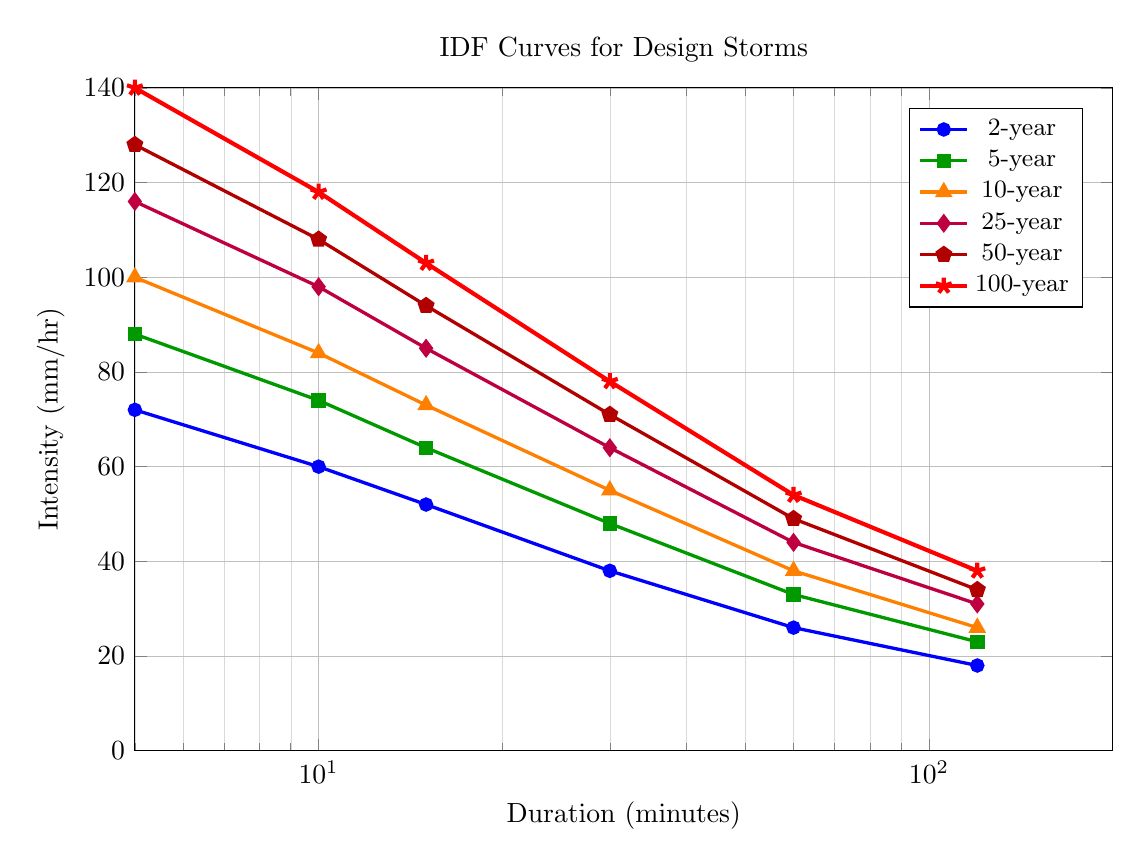
\begin{tikzpicture}
\begin{semilogxaxis}[
    width=14cm,
    height=10cm,
    xlabel={Duration (minutes)},
    ylabel={Intensity (mm/hr)},
    xmin=5, xmax=200,
    ymin=0, ymax=140,
    grid=both,
    grid style={line width=.1pt, draw=gray!30},
    major grid style={line width=.2pt,draw=gray!50},
    legend pos=north east,
    legend style={font=\small},
    title={IDF Curves for Design Storms}
]

% 2-year curve
\addplot[color=blue, line width=1.2pt, mark=*, mark size=2pt] coordinates {
    (5,72) (10,60) (15,52) (30,38) (60,26) (120,18)
};
\addlegendentry{2-year}

% 5-year curve
\addplot[color=green!60!black, line width=1.2pt, mark=square*, mark size=2pt] coordinates {
    (5,88) (10,74) (15,64) (30,48) (60,33) (120,23)
};
\addlegendentry{5-year}

% 10-year curve
\addplot[color=orange, line width=1.2pt, mark=triangle*, mark size=2.5pt] coordinates {
    (5,100) (10,84) (15,73) (30,55) (60,38) (120,26)
};
\addlegendentry{10-year}

% 25-year curve
\addplot[color=purple, line width=1.2pt, mark=diamond*, mark size=2.5pt] coordinates {
    (5,116) (10,98) (15,85) (30,64) (60,44) (120,31)
};
\addlegendentry{25-year}

% 50-year curve
\addplot[color=red!70!black, line width=1.2pt, mark=pentagon*, mark size=2.5pt] coordinates {
    (5,128) (10,108) (15,94) (30,71) (60,49) (120,34)
};
\addlegendentry{50-year}

% 100-year curve
\addplot[color=red, line width=1.5pt, mark=star, mark size=3pt] coordinates {
    (5,140) (10,118) (15,103) (30,78) (60,54) (120,38)
};
\addlegendentry{100-year}

\end{semilogxaxis}
\end{tikzpicture}
\end{center}

\textbf{Question 1 (3 marks):} From the IDF curve, determine the rainfall intensity for a 25-year return period storm with 30-minute duration.

\vspace{2cm}

\textbf{Question 2 (5 marks):} A commercial parking lot has the following characteristics:
\begin{itemize}[nosep]
    \item Drainage area: 1.8 hectares
    \item Runoff coefficient: 0.80
    \item Time of concentration: 15 minutes
    \item Design standard: 10-year return period
\end{itemize}

Using the IDF curve and the rational method $Q = \frac{1}{3600} \times C \times I \times A$ (where $I$ is in mm/hr, $A$ is in m$^2$), calculate the peak discharge in L/s.

\vspace{7cm}

\textbf{Question 3 (3 marks):} Compare the rainfall intensities for a 15-minute storm with return periods of 10 years and 100 years. Calculate the percentage increase from the 10-year to the 100-year event.

\vspace{3cm}

\textbf{Question 4 (4 marks):} Based on the IDF curves, explain why the intensity decreases as the duration increases for any given return period. Provide a physical interpretation relevant to storm characteristics.

\vspace{3cm}

\newpage

\subsection*{B.2: Frequency Analysis Plot (10 marks)}

\begin{center}
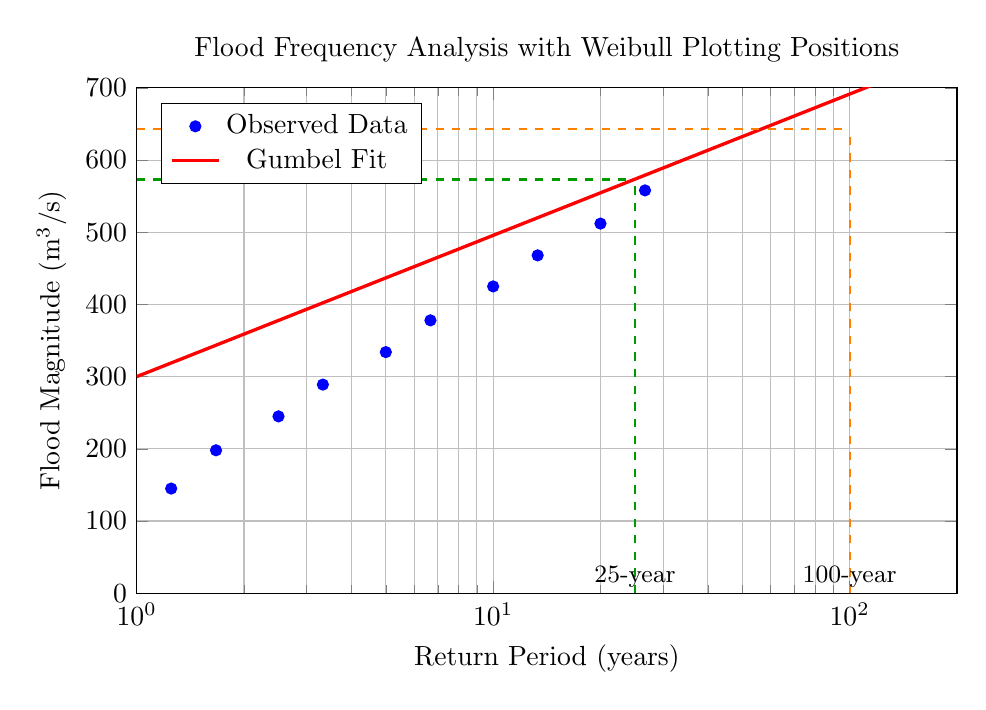
\begin{tikzpicture}
\begin{semilogxaxis}[
    width=12cm,
    height=8cm,
    xlabel={Return Period (years)},
    ylabel={Flood Magnitude (m$^3$/s)},
    xmin=1, xmax=200,
    ymin=0, ymax=700,
    grid=both,
    legend pos=north west,
    title={Flood Frequency Analysis with Weibull Plotting Positions}
]

% Observed data points (Weibull positions)
\addplot[only marks, mark=*, mark size=2pt, color=blue] coordinates {
    (1.25,145) (1.67,198) (2.5,245) (3.33,289) (5,334)
    (6.67,378) (10,425) (13.33,468) (20,512) (26.67,558)
};
\addlegendentry{Observed Data}

% Fitted Gumbel line
\addplot[color=red, line width=1.2pt, domain=1:200, samples=100]
    {300 + 85*ln(x)};
\addlegendentry{Gumbel Fit}

% Design event markers
\draw[dashed, thick, green!60!black] (axis cs:25,0) -- (axis cs:25,573);
\draw[dashed, thick, green!60!black] (axis cs:1,573) -- (axis cs:25,573);
\node[below] at (axis cs:25,50) {\small 25-year};

\draw[dashed, thick, orange] (axis cs:100,0) -- (axis cs:100,643);
\draw[dashed, thick, orange] (axis cs:1,643) -- (axis cs:100,643);
\node[below] at (axis cs:100,50) {\small 100-year};

\end{semilogxaxis}
\end{tikzpicture}
\end{center}

\textbf{Question (10 marks):} Based on the flood frequency analysis plot:
\begin{enumerate}[label=\alph*)]
    \item Read the 25-year design flood from the Gumbel fit. State the peak discharge value. (2 mark)
    \item Read the 100-year design flood from the Gumbel fit. State the peak discharge value. (2 mark)
    \item Calculate the factor of safety: How many times larger is the 100-year flood compared to the 25-year flood? (2 mark)
    \item Does the Gumbel distribution provide a good fit to the observed data (blue points)? Explain by commenting on the alignment between the red line and the data points. (4 marks)
\end{enumerate}

\vspace{3cm}

\newpage

\section*{Section C: Numerical Problems (30 marks)}

\subsection*{Problem 1: Weibull Analysis and Return Periods (8 marks)}

You have 30 years of annual maximum rainfall data. The 4th largest event recorded was 85 mm.

\begin{enumerate}[label=\alph*)]
    \item Calculate the Weibull plotting position $P$ for this event using $P = \frac{m}{n+1}$. (3 marks)
    \item Calculate the return period $T$ for this event. (2 marks)
    \item What is the annual exceedance probability for this event? (2 marks)
    \item In practical engineering terms, explain what this return period means. (1 mark)
\end{enumerate}

\vspace{8cm}

\subsection*{Problem 2: Risk and Reliability Analysis (8 marks)}

A storm water detention pond is designed for a 50-year return period storm with an expected service life of 30 years.

\begin{enumerate}[label=\alph*)]
    \item Calculate the annual exceedance probability $P$. (2 marks)
    \item Calculate the lifetime risk $R$ using $R = 1-(1-P)^n$. (3 marks)
    \item Calculate the reliability (Rel). (2 marks)
    \item If the acceptable risk for this type of facility is 30\%, does this design meet the criterion? (1 mark)
\end{enumerate}

\vspace{8cm}

\newpage

\subsection*{Problem 3: GEV Distribution Application (7 marks)}

A GEV distribution has been fitted to annual maximum flood data with the following parameters:
\begin{itemize}[nosep]
    \item Shape parameter: $\xi = +0.20$
    \item Location parameter: $\mu = 450$ m$^3$/s
    \item Scale parameter: $\sigma = 120$ m$^3$/s
\end{itemize}

\begin{enumerate}[label=\alph*)]
    \item What type of GEV distribution is this (Gumbel, Fréchet, or Weibull)? (2 marks)
    \item What does this shape parameter tell you about the tail behavior and extreme events? (2 marks)
    \item For engineering design, what implications does this positive shape parameter have? Should you be more or less conservative? (3 marks)
\end{enumerate}

\vspace{7cm}

\subsection*{Problem 4: IDF Application with Disaggregation (7 marks)}

For a location, the 60-minute annual maximum rainfall with a 50-year return period is 85 mm. Using NOAA temporal scaling ratios:

\begin{center}
\begin{tabular}{cc}
\toprule
Duration & NOAA Ratio \\
\midrule
5-min & 0.29 \\
15-min & 0.57 \\
30-min & 0.79 \\
60-min & 1.00 \\
\bottomrule
\end{tabular}
\end{center}

\begin{enumerate}[label=\alph*)]
    \item Calculate the 15-minute rainfall depth for the 50-year event. (2 marks)
    \item Calculate the rainfall intensity (mm/hr) for this 15-minute duration. (2 marks)
    \item Calculate the 30-minute rainfall depth for the 50-year event. (2 marks)
    \item Which duration (15-min or 30-min) has higher intensity? Explain why. (1 mark)
\end{enumerate}

\vspace{7cm}

\newpage

\section*{Section D: Short Answer/Theoretical Questions (15 marks)}

\subsection*{Question 1: Hydrological and Hydrodynamic Modelling (5 marks)}

Define modeling in the context of water resources engineering. Provide a few examples of models and explain applications of modeling. 

\vspace{5cm}

\subsection*{Question 2: Design of hydraulic structures (5 marks)}

As a design engineer, you have been assigned the task of planning and designing a new dam and reservoir system. Discuss briefly the key design considerations, including hydrological and hydraulic aspects. 

\vspace{5cm}

\subsection*{Question 3: Governing Equations in Open Channel Flow (5 marks)}

Explain the concept of open channel flow. Derive or state the governing equations and illustrate with practical examples.

\vspace{5cm}

\newpage

\section*{Formula Table}

\subsection*{Frequency Analysis}
\renewcommand{\arraystretch}{1.5}
\begin{tabular}{|l|l|l|}
\hline
\textbf{Formula} & \textbf{Description} & \textbf{Variables} \\
\hline
$P = \frac{m}{n+1}$ & Weibull plotting position & $m$ = rank, $n$ = total observations \\
$T = \frac{1}{P}$ & Return period & $T$ = return period (years) \\
$P = \frac{1}{T}$ & Annual exceedance probability & $P$ = probability \\
\hline
\end{tabular}

\subsection*{Risk and Reliability}
\begin{tabular}{|l|l|l|}
\hline
\textbf{Formula} & \textbf{Description} & \textbf{Variables} \\
\hline
$R = 1-(1-P)^n$ & Lifetime risk & $R$ = risk, $n$ = design life \\
$Rel = (1-P)^n$ & Reliability & $Rel$ = reliability \\
$R + Rel = 1$ & Risk-reliability relationship & \\
\hline
\end{tabular}

\subsection*{Probability Calculations}
\begin{tabular}{|l|l|l|}
\hline
\textbf{Formula} & \textbf{Description} & \textbf{Variables} \\
\hline
$0 \leq P \leq 1$ & Probability range & \\
$P(X \geq a) = 1 - F(a)$ & Exceedance probability & $F(x)$ = CDF \\
$P(a \leq X \leq b) = F(b) - F(a)$ & Interval probability & \\
$P(X \leq a) = F(a)$ & Non-exceedance probability & \\
\hline
\end{tabular}

\subsection*{IDF Curves and Rainfall}
\begin{tabular}{|l|l|l|}
\hline
\textbf{Formula} & \textbf{Description} & \textbf{Variables} \\
\hline
$I = \frac{P}{t}$ & Intensity from depth & $I$ = intensity (mm/hr), $P$ = depth (mm) \\
& & $t$ = duration (hours) \\
$I = \frac{P}{t_{min}} \times 60$ & Intensity (duration in min) & $t_{min}$ = duration (minutes) \\
$Q = \frac{1}{3600} \times C \times I \times A$ & Rational method & $Q$ = discharge (m$^3$/s), $C$ = runoff coeff \\
& (I in mm/hr, A in m$^2$) & $A$ = area (m$^2$) \\
$P_t = P_{60} \times Ratio_t$ & NOAA temporal scaling & $P_t$ = rainfall at duration $t$ \\
\hline
\end{tabular}

\subsection*{GEV Distribution}
\begin{tabular}{|l|l|l|}
\hline
\textbf{Shape Parameter} & \textbf{Type} & \textbf{Tail Behavior} \\
\hline
$\xi > 0$ & Fréchet (Type II) & Heavy tail - more extreme events \\
$\xi = 0$ & Gumbel (Type I) & Standard tail - normal extremes \\
$\xi < 0$ & Weibull (Type III) & Light tail - bounded extremes \\
\hline
\end{tabular}

\subsection*{NOAA Temporal Scaling Ratios}
\begin{tabular}{|l|c|}
\hline
\textbf{Duration} & \textbf{Typical Ratio} \\
\hline
5-minute & 0.29 \\
10-minute & 0.45 \\
15-minute & 0.57 \\
30-minute & 0.79 \\
60-minute & 1.00 \\
\hline
\end{tabular}

\subsection*{Statistical Measures}
\begin{tabular}{|l|l|l|}
\hline
\textbf{Formula} & \textbf{Description} & \textbf{Variables} \\
\hline
$\mu = \frac{1}{n}\sum_{i=1}^{n} x_i$ & Mean & $\mu$ = mean, $x_i$ = observations \\
$\sigma = \sqrt{\frac{1}{n-1}\sum_{i=1}^{n}(x_i-\mu)^2}$ & Standard deviation & $\sigma$ = standard deviation \\
$CV = \frac{\sigma}{\mu}$ & Coefficient of variation & $CV$ = coefficient of variation \\
\hline
\end{tabular}

\subsection*{Unit Conversions}
\begin{itemize}[nosep]
    \item 1 hectare = 10,000 m$^2$
    \item 1 m$^3$/s = 1000 L/s
    \item Intensity (mm/hr) = $\frac{\text{Depth (mm)}}{\text{Duration (hr)}}$
    \item To convert minutes to hours: divide by 60
    \item To convert hours to minutes: multiply by 60
\end{itemize}

\vspace{0.5cm}
\hrule
\vspace{0.3cm}
\begin{center}
\textbf{END OF EXAMINATION}
\end{center}

\end{document}
